Ben Trout

2015-01-23

Building

\begin{tabular}{|p{5cm}|p{5cm}|}
\hline
Linear Slides&
While Nick worked on fixing the spinner, moving it, and replacing bent pieces, I moved the linear slide around. I attached the linear slide the the side of the robot. With the help of David we attached a channel parallel with our back vertical side channel. The motor is mounted to this channel too. The linear slide system is the same as before screwed to this bar with it’s pulley system perfectly in line the the motor tip.
\\
\hline
Cardboard Proto&
Alex is going to make a polycarb guide tube, but he wanted a cardboard proto to show proof of concept and get exact dimensions for the actual guide tube. The guide tube is three sections of cardboard starting with the largest 7 1/2in length, 4in width, and 14in tall. Each width and length step down by 1/4 every smaller section. All three sections are 14in tall except the smallest which is 15in tall. The medium has two slots cut in it 1in from both edges. The largest sections has two screws that slide into these slots and as it is raised the screws will go up the slots till they catch and then the medium section will be raised with the large section. The smallest section is screwed to the base of the robot. 
\\
\hline
\end{tabular}

\section*{linear slides}
The whole goal of moving the linear slides was to allow us to push the guide tube all the way to the back of the robot. This would allow us to push the spinner back a couple holes and by redoing the intake we were able to put a support bar across the front middle of our robot for support. Setting up and screwing the linear slide to the side of the robot was the easy part. What was hard was all the things that it got in the way of. Filip had to move all the motors to the very back of the robot as the linear slide was hitting the motor. I also had a fun time figuring out the new placement of the motor. We wanted it parallel with the bar, but at the same time in line with the pulleys. We also had to stay inside our size limit. I ended up going with the motor perpendicular with the pulleys, but in line. This would allow us to stay inside the size and get the least amount of counterforce on the motor. 

\section*{Guidetube Proto}
David was initially in charge of protoing the guide tube and came up with the idea of having three separate sections that slide into each other. I rolled with this idea and prototyped a cardboard tube. Our spinner is 6.5 in wide so I made our smallest guide section 7in wide. Our deflector is 4 in length, so I made the largest section 4 inches in length. The rest of making the cardboard sections was easy because the cardboard and polycarb is 1/8 thick so I just stepped each section’s length and width down by 1/4. I came across a couple problems while making the prototype though. First if you step each sections length down by 1/4 it causes a lot of friction as the sections have a lot of contact. For the final alex will give an extra 1/16 on both sides to make sure this doesn’t happen. I made each section by cutting out a piece in cardboard the size of the section’s perimeters; then I measured out each length and width twice and scored those lines. The cardboard then folded up into a perfect sized box. The only problem is for one width of each section you have to make it 1/8 in smaller because as it folds the length rests on top of the width which adds an extra 1/8 inch. I had to make the smaller section an extra in large because the small section fits between our wheels while the medium and large rest on top of the wheels. Adding this extra inch allows us to drill the small section stationary to the bottom of our robot base.

\begin{center}
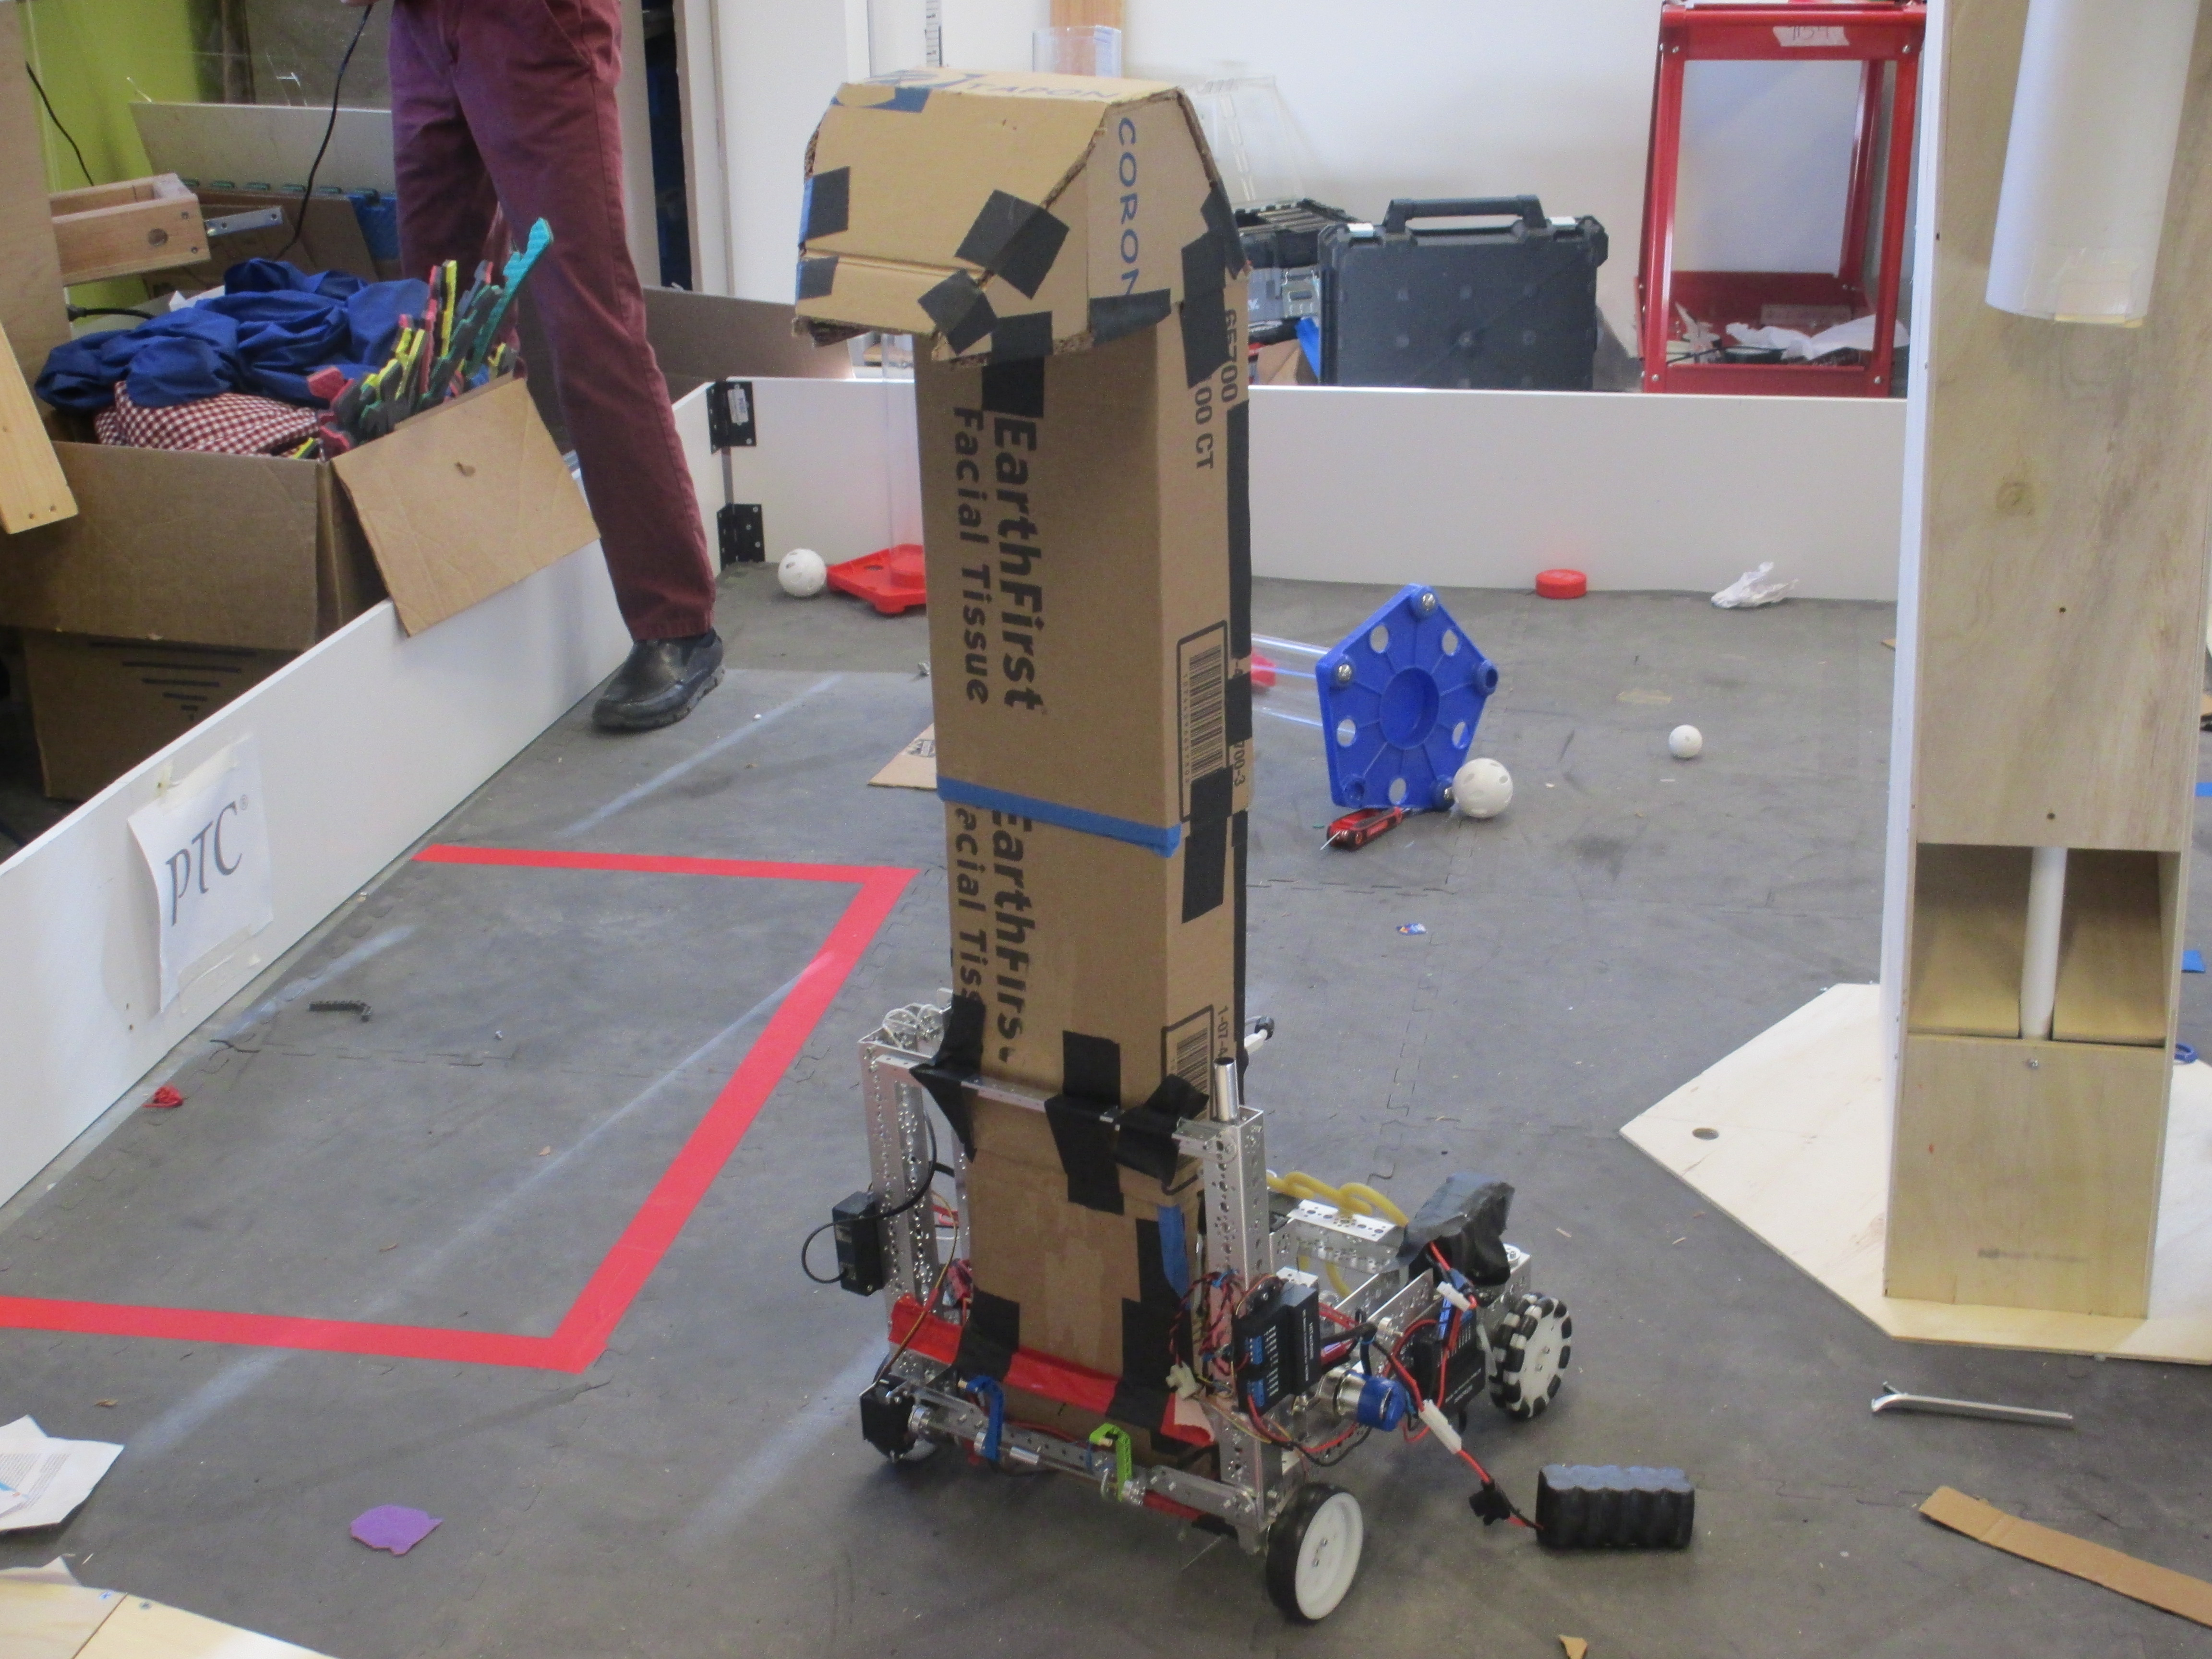
\includegraphics[width=10cm]{./Entries/Images/CardboardProto.JPG}
\end{center}

Cardboard Prototype

